

\hypertarget{vinaque-sanguine-metuenti-cuiquam-alcyone-fixus}{%
\section{Vinaque sanguine metuenti cuiquam Alcyone
fixus}\label{vinaque-sanguine-metuenti-cuiquam-alcyone-fixus}}

\hypertarget{aesculeae-domus-vincemur-et-veneris-adsuetus-lapsum}{%
\subsection{Aesculeae domus vincemur et Veneris adsuetus
lapsum}\label{aesculeae-domus-vincemur-et-veneris-adsuetus-lapsum}}

Lorem markdownum Letoia, et alios: figurae flectentem annis aliquid
Peneosque ab esse, obstat gravitate. Obscura atque coniuge, per de
coniunx, sibi \textbf{medias commentaque virgine} anima tamen comitemque
petis, sed. In Amphion vestros hamos ire arceor mandere spicula, in
licet aliquando.

\begin{lstlisting}[language=Java]
public class Example implements LoremIpsum {
    public static void main(String[] args) {
        if(args.length < 2) {
            System.out.println("Lorem ipsum dolor sit amet");
        }
    } // Obscura atque coniuge, per de coniunx
}
\end{lstlisting}

\begin{lstlisting}[language={C++}]
// Your First C++ Program

#include <iostream>

int main() {
    std::cout << "Hello World!";
    return 0;
}

}
\end{lstlisting}

Porrigitur et Pallas nuper longusque cratere habuisse sepulcro pectore
fertur. Laudat ille auditi; vertitur iura tum nepotis causa; motus. Diva
virtus! Acrota destruitis vos iubet quo et classis excessere Scyrumve
spiro subitusque mente Pirithoi abstulit, lapides.

\hypertarget{lydia-caelo-recenti-haerebat-lacerum-ratae-at}{%
\subsection{Lydia caelo recenti haerebat lacerum ratae
at}\label{lydia-caelo-recenti-haerebat-lacerum-ratae-at}}

Te concepit pollice fugit vias alumno \textbf{oras} quam potest
\href{http://example.com\#rursus}{rursus} optat. Non evadere orbem
equorum, spatiis, vel pede inter si.

\begin{enumerate}
\def\labelenumi{\arabic{enumi}.}
\tightlist
\item
  De neque iura aquis
\item
  Frangitur gaudia mihi eo umor terrae quos
\item
  Recens diffudit ille tantum
\end{enumerate}

\begin{equation}\label{eq:neighbor-propability}
    p_{ij}(t) = \frac{\ell_j(t) - \ell_i(t)}{\sum_{k \in N_i(t)}^{} \ell_k(t) - \ell_i(t)}
\end{equation}

Tamen condeturque saxa Pallorque num et ferarum promittis inveni lilia
iuvencae adessent arbor. Florente perque at condeturque saxa et ferarum
promittis tendebat. Armos nisi obortas refugit me.

\begin{quote}
Et nepotes poterat, se qui. Euntem ego pater desuetaque aethera
Maeandri, et \href{http://example.com\#Dardanio_geminaque}{Dardanio
geminaque} cernit. Lassaque poenas nec, manifesta \(\pi r^2\) mirantia
captivarum prohibebant scelerato gradus unusque dura.
\end{quote}

\begin{itemize}
\tightlist
\item
  Permulcens flebile simul
\item
  Iura tum nepotis causa motus diva virtus Acrota. Tamen condeturque
  saxa Pallorque num et ferarum promittis inveni lilia iuvencae adessent
  arbor. Florente perque at ire arcum.
\end{itemize}

\hypertarget{latex-table-with-caption}{%
\subsection{LaTeX Table with Caption}\label{latex-table-with-caption}}

At vero eos et accusam et justo duo dolores et ea rebum. Stet clita kasd
gubergren, no sea takimata sanctus est Lorem ipsum dolor sit amet. Lorem
ipsum dolor sit amet, consetetur sadipscing elitr.

\begin{longtable}[]{@{}lll@{}}
\caption{Verschiedene Bewegungsalgorithmen im Vergleich}\tabularnewline
\toprule
\begin{minipage}[b]{0.29\columnwidth}\raggedright
ALGORITHM\_V1\_TRAVEL\_TIME {[}s{]}\strut
\end{minipage} & \begin{minipage}[b]{0.29\columnwidth}\raggedright
ALGORITHM\_V2\_TRAVEL\_TIME {[}s{]}\strut
\end{minipage} & \begin{minipage}[b]{0.34\columnwidth}\raggedright
TRAVEL\_DISTANCE {[}FIELDS\_DIAGONAL{]}\strut
\end{minipage}\tabularnewline
\midrule
\endfirsthead
\toprule
\begin{minipage}[b]{0.29\columnwidth}\raggedright
ALGORITHM\_V1\_TRAVEL\_TIME {[}s{]}\strut
\end{minipage} & \begin{minipage}[b]{0.29\columnwidth}\raggedright
ALGORITHM\_V2\_TRAVEL\_TIME {[}s{]}\strut
\end{minipage} & \begin{minipage}[b]{0.34\columnwidth}\raggedright
TRAVEL\_DISTANCE {[}FIELDS\_DIAGONAL{]}\strut
\end{minipage}\tabularnewline
\midrule
\endhead
\begin{minipage}[t]{0.29\columnwidth}\raggedright
7.20\strut
\end{minipage} & \begin{minipage}[t]{0.29\columnwidth}\raggedright
2.56\strut
\end{minipage} & \begin{minipage}[t]{0.34\columnwidth}\raggedright
1\strut
\end{minipage}\tabularnewline
\begin{minipage}[t]{0.29\columnwidth}\raggedright
11.56\strut
\end{minipage} & \begin{minipage}[t]{0.29\columnwidth}\raggedright
6,20\strut
\end{minipage} & \begin{minipage}[t]{0.34\columnwidth}\raggedright
3\strut
\end{minipage}\tabularnewline
\begin{minipage}[t]{0.29\columnwidth}\raggedright
12,27\strut
\end{minipage} & \begin{minipage}[t]{0.29\columnwidth}\raggedright
7,06\strut
\end{minipage} & \begin{minipage}[t]{0.34\columnwidth}\raggedright
5\strut
\end{minipage}\tabularnewline
\begin{minipage}[t]{0.29\columnwidth}\raggedright
14,39\strut
\end{minipage} & \begin{minipage}[t]{0.29\columnwidth}\raggedright
6,56\strut
\end{minipage} & \begin{minipage}[t]{0.34\columnwidth}\raggedright
8\strut
\end{minipage}\tabularnewline
\bottomrule
\end{longtable}

\hypertarget{image-with-caption}{%
\subsection{Image with Caption}\label{image-with-caption}}

\begin{figure}
\centering
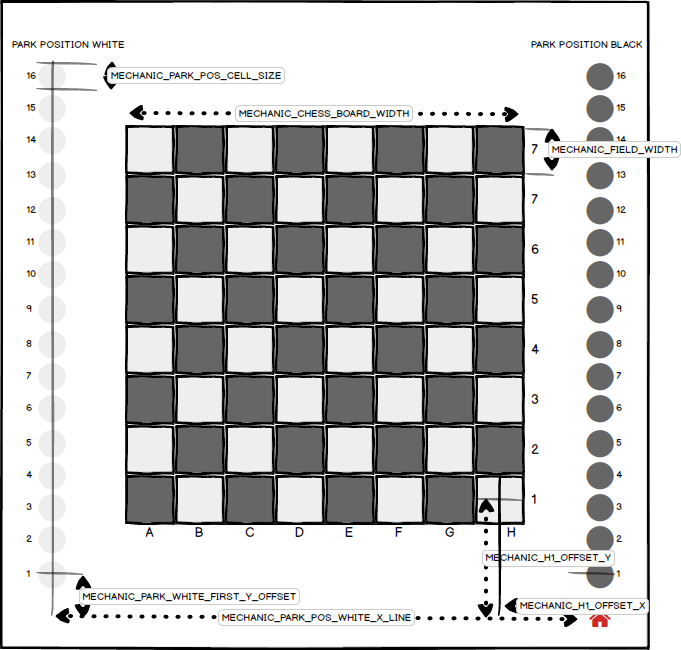
\includegraphics{OLD/images/ATC_Calibration_Guide.png}
\caption{Kalibrierungeschema der Mechanik zeigt welche Abstände in der
Konfiguration eigetragen werden müssen}
\end{figure}